\documentclass[conference]{IEEEtran}
\IEEEoverridecommandlockouts

\usepackage{cite}
\usepackage{amsmath,amssymb,amsfonts}
\usepackage{graphicx}
\usepackage{textcomp}
\usepackage{xcolor}
\usepackage{booktabs}
\usepackage{array}
\usepackage{algorithm}
\usepackage{algpseudocode}
\usepackage{dblfloatfix}
\usepackage{float}

\graphicspath{{images/}}

\begin{document}

\title{Min-Conflicts Local Search on a Terrain Map-Coloring CSP}

\author{
    \IEEEauthorblockN{Jacob A. Geldbach}
    \IEEEauthorblockA{
        \textit{College of Engineering: CS} \\
        \textit{University of Idaho} \\
        Moscow Idaho, United States \\
        geld8788@vandals.uidaho.edu
    }
}

\maketitle

\begin{abstract}
    Min-Conflicts is a local search algorithm useful for solving constraint satisfaction problems (CSPs). In this project, Min-Conflicts was applied to a terrain detailed grid map coloring CSP, where different terrains acted as the variables and the constraints were related to which terrains could be adjacent to each other. The algorithm was tested on 5 differnt map sizes, with and without diagonal neighbors.
\end{abstract}

\begin{IEEEkeywords}
    Local Search, Contraint Satisfaction Problem, Min-Conflicts, Map Coloring, Convergence
\end{IEEEkeywords}

% =======================================================
\section{Introduction}
    In this project, the Min-Conflicts algorithm was successfully implemented in order to solve a terrain map-coloring CSP problem. The terrains were represented as a grid of cells which is generated randomly and represented in real time as the algorithm runs. The python process uses the Pygame visualization library to display the initial random terrain assignment for the inputted map size, then continues to display an update of the grid every 50 steps until either the algorithm finds a solution or the stopping criterion is met. The constraints for this problem are the adjacency rules for the terrains defined below in Table \ref{tab:adjacency}. This projects python process has the ability to run headless without generating the visualization at all, this was useful for the data gathering portion of the project where I ran 16 trials for each map size.The ability to run the algorithm headless allowed for the trials to be ran in parallel and gather the data much faster as on the larger map sizes the Min-Conflicts algorith took a long time to either converge or reach the stopping criterion, the reason for this discussed in the below sections. The algorithm was successful in converging on a solution in all 10 conditions tested, and the data gathered allowed for a clear representation of how this CSPs time complexity scales with the size of the map or the number of variables constrained.

% -------------------------------------------------------
\begin{table}[H]
\caption{Terrain Adjacency Compatibility Matrix}
\begin{center}
\footnotesize
\setlength{\tabcolsep}{4pt}
\begin{tabular}{l c c c c c c}
\toprule
\textbf{Terrain} & \rotatebox{90}{Water} & \rotatebox{90}{Beach} & \rotatebox{90}{Lowland} & \rotatebox{90}{Forest} & \rotatebox{90}{Hills} & \rotatebox{90}{Mountains} \\
\midrule
Water     & \checkmark & \checkmark & $\times$   & $\times$   & $\times$   & $\times$   \\
Beach     & \checkmark & \checkmark & \checkmark & $\times$   & $\times$   & $\times$   \\
Lowland   & $\times$   & \checkmark & \checkmark & \checkmark & $\times$   & $\times$   \\
Forest    & $\times$   & $\times$   & \checkmark & \checkmark & \checkmark & $\times$   \\
Hills     & $\times$   & $\times$   & $\times$   & \checkmark & \checkmark & \checkmark \\
Mountains & $\times$   & $\times$   & $\times$   & $\times$   & \checkmark & \checkmark \\
\bottomrule
\end{tabular}
\label{tab:adjacency}
\end{center}
\footnotesize A \checkmark\ marks a legal adjacency (elevation differs by at most one step); $\times$ marks a constraint violation. Every terrain is trivially compatible with itself.
\end{table}

% =======================================================
\section{Algorithm Description}
% Explain min-conflicts in your own words. Cover:
%   - Core idea: how it decides WHICH cell to change and WHAT value to assign.
%   - Why a random complete assignment differs from building a solution incrementally.
%   - Completeness: is it guaranteed to find a solution if one exists? Why / why not?
%   - Your stopping criterion: what it is, why you chose it, effect on failure counts.
%   - Anything non-standard or tricky you implemented.
Min-Conflicts being a local search algorithm starts in a problem search space by randomly choosing a potential solution, in this case that is a complete assignment of values to the variables. The algorithm must then "grade" or determine how many constraint violations this grid state has, this is where the majority of the time complexity comes from. The algorithm must first iterate over each cell in the grid and check each of it's neighbors to see if any of the contraints are violated, each cell with a constraint violation is then added to a list of conflicted cells. A conflicted cell is then chosen at random and the algorithm iterates over all the possible values for that cell and determines which value would improve the overall conflicted state of the current grid state. These two steps result in time complexities described by $O(n*d)$ and $O(k*d)$ respectively, where $n$ is the number of cells or variables, $d$ is the number of neighbors for each cell, and $k$ is the number of possible values for each variable or terrains each cell can be colored. Due to in this problem $k$ being a constant value of 5, and $d$ being a constant value of 4 or 8, the time complexity for the step of finding a new terrain for the chosen conflicted cell is negligible and considered constant $O(1)$. Min-Conflicts being a local search algorithm benefits from the memory efficiency of only storing the current state of the grid and that of the candidate state being tested, therefore the space complexity is $O(n)$ where $n$ is the number of cells on the grid. Min-Conflicts is not guaranteed to find a solution if one exists, this is due to there before possible plateaus or local maximum in the search space where the algorithm can get stuck and not be able to find a better solution. Due to this fact a stopping criterion is essential to prevent the algorithm from running indefinitely. In this project I chose a stopping criterion of steps since improvement. Essentially if a certain number of iterations or steps have passed without the algorithm finding a better solution, i.e. decreasing the total number of conflicts, then the algorithm will stop and report a failure to converge. Due to the number of variable scaling of Min-Conflicts time complexity, I also have the stopping criterion of steps since improvement scaling with the size of the grid, where $steps_since_improvement = w * h$ where $w$ and $h$ are the width and height of the grid. I chose this so that the algorithm has a fair chance to converge on larger variable conditions and so that algorithm could stop when in a clear plateau or local maximum instead of continuing on for 10s of thousands of more iterations until a static maximum number of steps criteria was hit. A key benefit of Min-Conflicts shows itself in this problem space especially in the larger map size conditions, and it lies in the first step of starting from a random state of values assigned to the variables. By starting in this random potential solution, the exponential time complexity of building a solution to the CSP incrementally (really finding the solution) by traversing a tree of potential value assignments is able to be avoided. Restated, although this approach is complete, to incrementally build a grid of terrains that do not have any conflicts would be of time and space complexity of $O(k^n)$ where $n$ is the total number of cells in the grid and $k$ is the 6 terrain choices. Take the 200x200 largest grid condition, where $n = 40,000$, to incrementally find the solution the time and space complexities are $O(6^40,0000)$, practically $INF$ in terms of even modern day computers. In other words, Min-Conflicts sacrificing completeness, allows for that condition in practice to become solvable. In this project, a greedy flag or non-classic Min-Conflicts argument was added which would instruct the algorithm to pick the next conflicted cell from a list of the \textit{most} conflicted cells (i.e. cells were sorted by the number of neighbors they were conflicting with) instead of picking \textit{any} conflicted cell. The thought process behind this addition was that by tackling the most conflicted cells first it may speed up time or lessen the number of steps before convergence. Counter-intuitively this caused the algorithm to plateau more often, which will be discussed in more depth in later sections.



% =======================================================
\section{Results}

% -------------------------------------------------------
\subsection{Map Visualizations}
% Before/after pair for at least one map size, with a legend of terrain colors.
% Drop your PNGs into images/ and rename below (or change the filenames here).

\begin{figure*}[t]
\centering
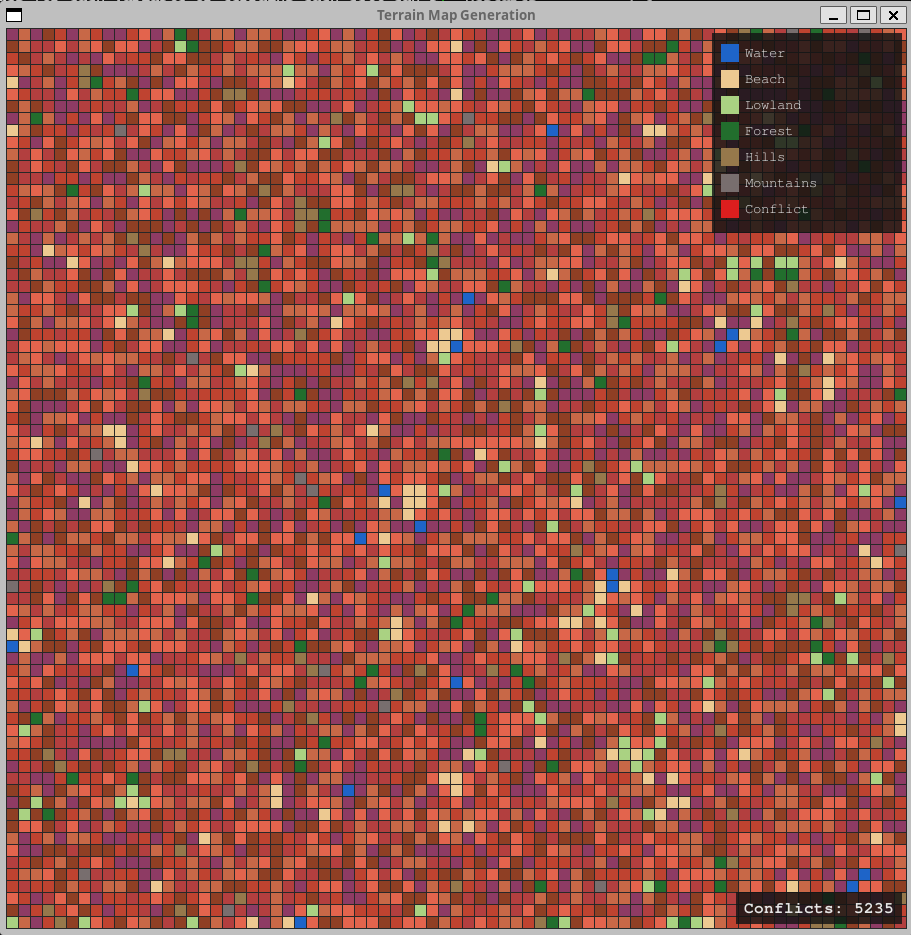
\includegraphics[width=0.42\linewidth]{map_before}
\hfil
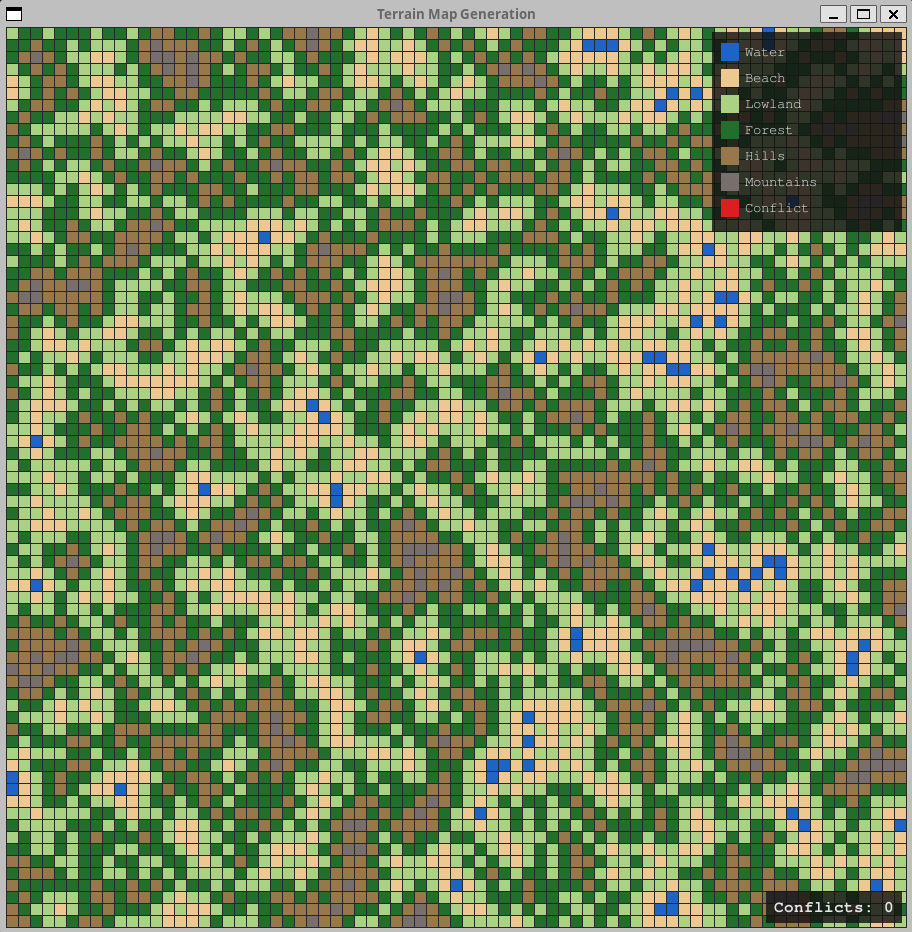
\includegraphics[width=0.42\linewidth]{map_after}
\caption{ Left: Beginning random terrain assignments for the the 75x75 grid size
          Right: Successful convergence of a solution
         }
\label{fig:before_after}
\end{figure*}

% TODO: briefly describe what changed between the before and after images.


% -------------------------------------------------------
\subsection{Results Table}
% Averages over 16 trials per condition. Fill the three data columns.
% Failures: enter 0 if a condition never failed.
% Avg. Iterations: enter N/A if a condition never succeeded.

\begin{table*}[t]
\caption{Min-Conflicts --- Convergence Results (16 trials per condition)}
\begin{center}
\footnotesize
\setlength{\tabcolsep}{6pt}
\begin{tabular}{c c >{\centering\arraybackslash}p{1.4in} >{\centering\arraybackslash}p{1.3in} >{\raggedright\arraybackslash}p{1.8in}}
\toprule
\textbf{Map Size} & \textbf{Diagonals} & \textbf{\shortstack{Avg. Iterations\\(success)}} & \textbf{\shortstack{Failures\\(out of 16 trials)}} & \textbf{Stopping Criterion} \\
\midrule
50$\times$50   & Off & 4892  & 2  & steps without improvement \\
50$\times$50   & On  & 5752  & 0  & steps without improvement \\
75$\times$75   & Off & 11225 & 3  & steps without improvement \\
75$\times$75   & On  & 12939 & 0  & steps without improvement \\
100$\times$100 & Off & 19877 & 3  & steps without improvement \\
100$\times$100 & On  & 23038 & 0  & steps without improvement \\
150$\times$150 & Off & 44937 & 4  & steps without improvement \\
150$\times$150 & On  & 52045 & 0  & steps without improvement \\
200$\times$200 & Off & 79852 & 12 & steps without improvement \\
200$\times$200 & On  & 92672 & 0  & steps without improvement \\
\bottomrule
\end{tabular}
\label{tab:results}
\end{center}
\end{table*}


% -------------------------------------------------------
\subsection{Convergence Graph}
% Map size vs. average iterations to convergence, one series per diagonals setting.
% Drop convergence.png into images/. Note any frequent-failure conditions near the graph.

\begin{figure}[H]
\centering
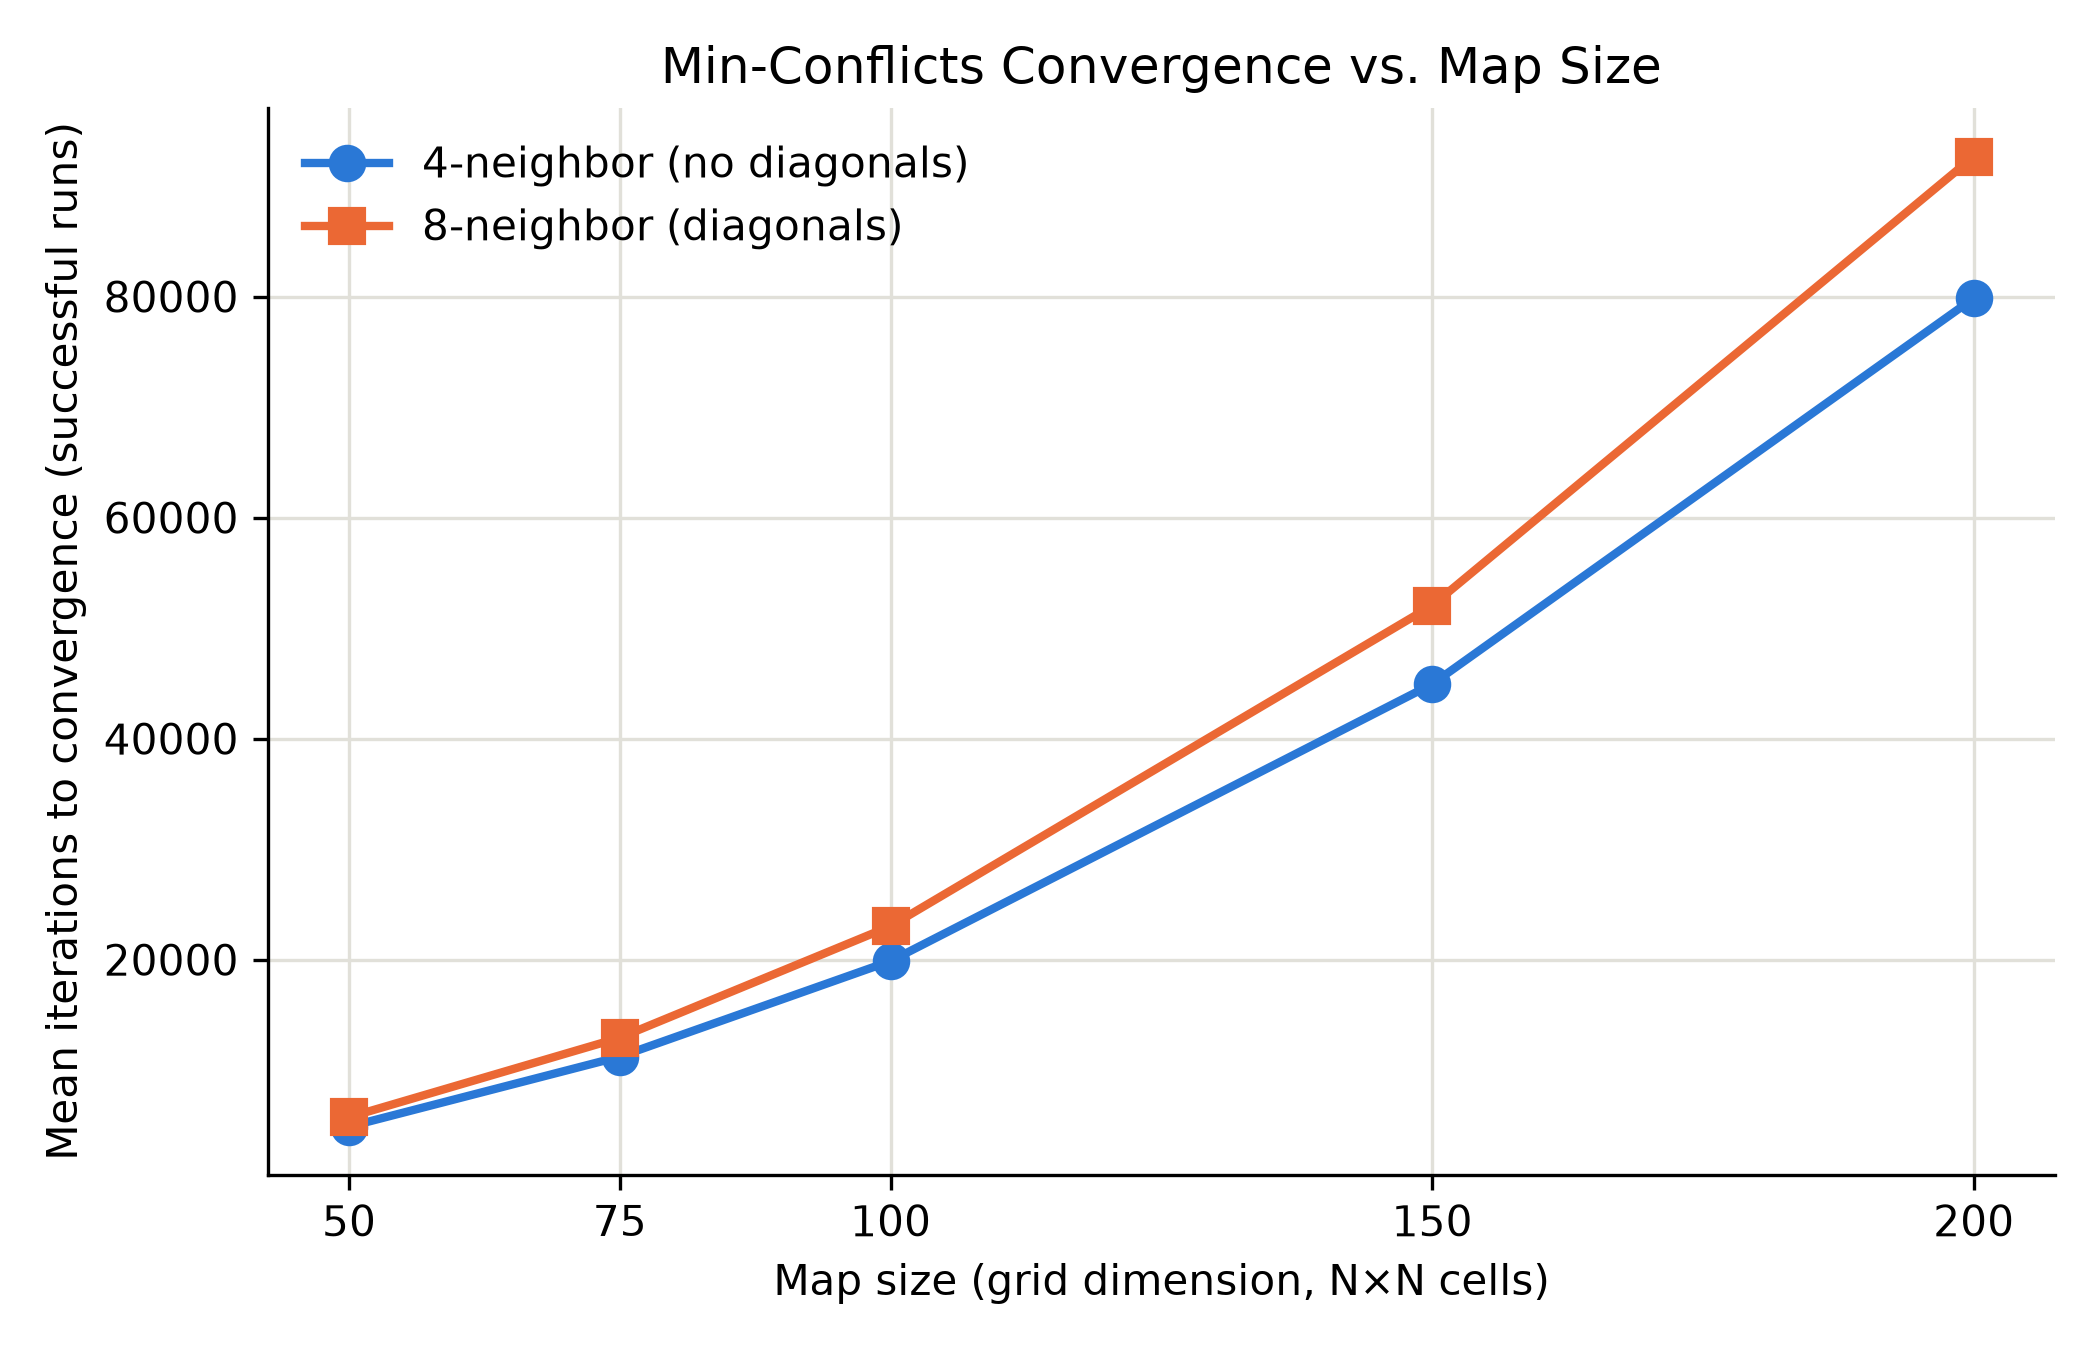
\includegraphics[width=\linewidth]{convergence}
\caption{% TODO: caption. Map size vs. mean iterations to convergence (successful runs),
         % 4-neighbor vs. 8-neighbor. Note conditions with frequent failures.
         }
\label{fig:convergence}
\end{figure}


% =======================================================
\section{Discussion}
% Synthesize results using specific numbers from the table and graph. Address:
%   - How did convergence time scale with map size? Linear / faster / slower than linear?
%   - Effect of diagonal neighbors on convergence and failure rates. Was it expected?
%   - Any runs that got "stuck" making little/no progress? What was happening?
%   - What the before/after images tell you about how the algorithm works;
%     is the after map geographically plausible? Why / why not?
%   - How min-conflicts compares conceptually to the Project 1 search algorithms;
%     key differences in how each approaches the problem.


% =======================================================
\section*{Use of AI}

\subsection*{Coding}
% Which tool(s) / model(s), and how used (initial code, debugging, APIs, tests, other).


\subsection*{What Worked and Didn't Work}
% How useful AI assistance was for coding and why; anything that didn't work well.


\subsection*{Writing}
% Whether AI helped draft/revise the write-up, how, and how you ensured the final
% text reflects your own understanding. (Write N/A if you used none.)


\end{document}
